\subsection{Brain Data}
We use the fMRI recordings of human subjects while they solve AUT and OCT tasks from \citet{beaty2018robust}. This brain dataset contains fMRI recordings from $170$ healthy subjects. Subjects were given the following instructions, respectively, for each task, and then were shown a stimulus one at a time. 

\begin{prompt}[title={AUT Instructions}, label=prompt:aut_instructions]
\begin{Verbatim}[breaklines, breaksymbol={}]
Think of creative uses for objects. Report the most original idea. Keep thinking of ideas during the thinking period. Quality is more important than quantity.
\end{Verbatim}
\end{prompt}

\begin{prompt}[title={OCT Instructions}, label=prompt:oct_instructions]
\begin{Verbatim}[breaklines, breaksymbol={}]
Think of the physical properties of objects. Report the most prominent characteristic. Keep thinking of ideas during the thinking period.
\end{Verbatim}
\end{prompt}

After a brief period of thinking, their responses, along with fMRI recordings, were collected for each stimulus. In total, subjects solved both tasks for $46$ stimuli, where each subject was exposed to on average $23$ stimuli for each task. For example, given the stimulus \textit{``kite''}, one subject responded with \textit{``a paper to write on''} and \textit{``rectangular''} respectively for AUT and OCT tasks. 

We first perform data cleaning based on the subject responses and, as a result, remove data for $8$ participants who failed to follow the task instructions, failed to provide a response, or whose brain data were incompatible with others in the neural representation dimension. Next, we apply standard fMRI data preprocessing (e.g., removing confounders, detrending, standardizing, and signal filtering) using \texttt{nilearn}\footnote{https://nilearn.github.io} library, which results in ``clean'' (but raw) fMRI brain activations \citep{matthews2004functional}. Rather than using these raw activations, we follow standard practice and estimate single-trial beta maps using a General Linear Model (GLM) \citep{draper1998applied}, and conduct all subsequent brain-LLM alignment analyses on these estimated neural response patterns. We extracted brain data from across three functional brain networks using the \citet{yeo2011organization} parcellation: the Default Mode Network (DMN), the Frontoparietal Network (FPN), and the Somatomotor Network. The DMN and FPN were selected given their well-established roles in creative cognition \citep{beaty2016creative, luchini2025role, liu2024neural}, while the Somatomotor Network was selected given its limited involvement in higher-order cognitive processes, making it a suitable control network.

\subsection{Model Data}
We provide the same instructions\footnote{We only replace the word ``objects'' with the stimulus name since we evaluate language-only models.} and the stimuli to an LLM and extract its intermediate layer activations as the model representations of the stimuli. Prior brain-LLM alignment studies typically extract model representations for the input prompt alone, which is sufficient for passive language tasks where no generation occurs. However, this is not sufficient for our task, which involves active generation, so we extract representations at both the prompt stage and after the model has generated a response, allowing us to capture the full generative process that more closely mirrors the demands of the AUT task. We note that this setup is similar to \citet{kwon2024assessing} except that we investigate alignment both at the prompt and generation stage, while \citet{kwon2024assessing} only examines alignment at the generation stage.

\begin{figure}[t]
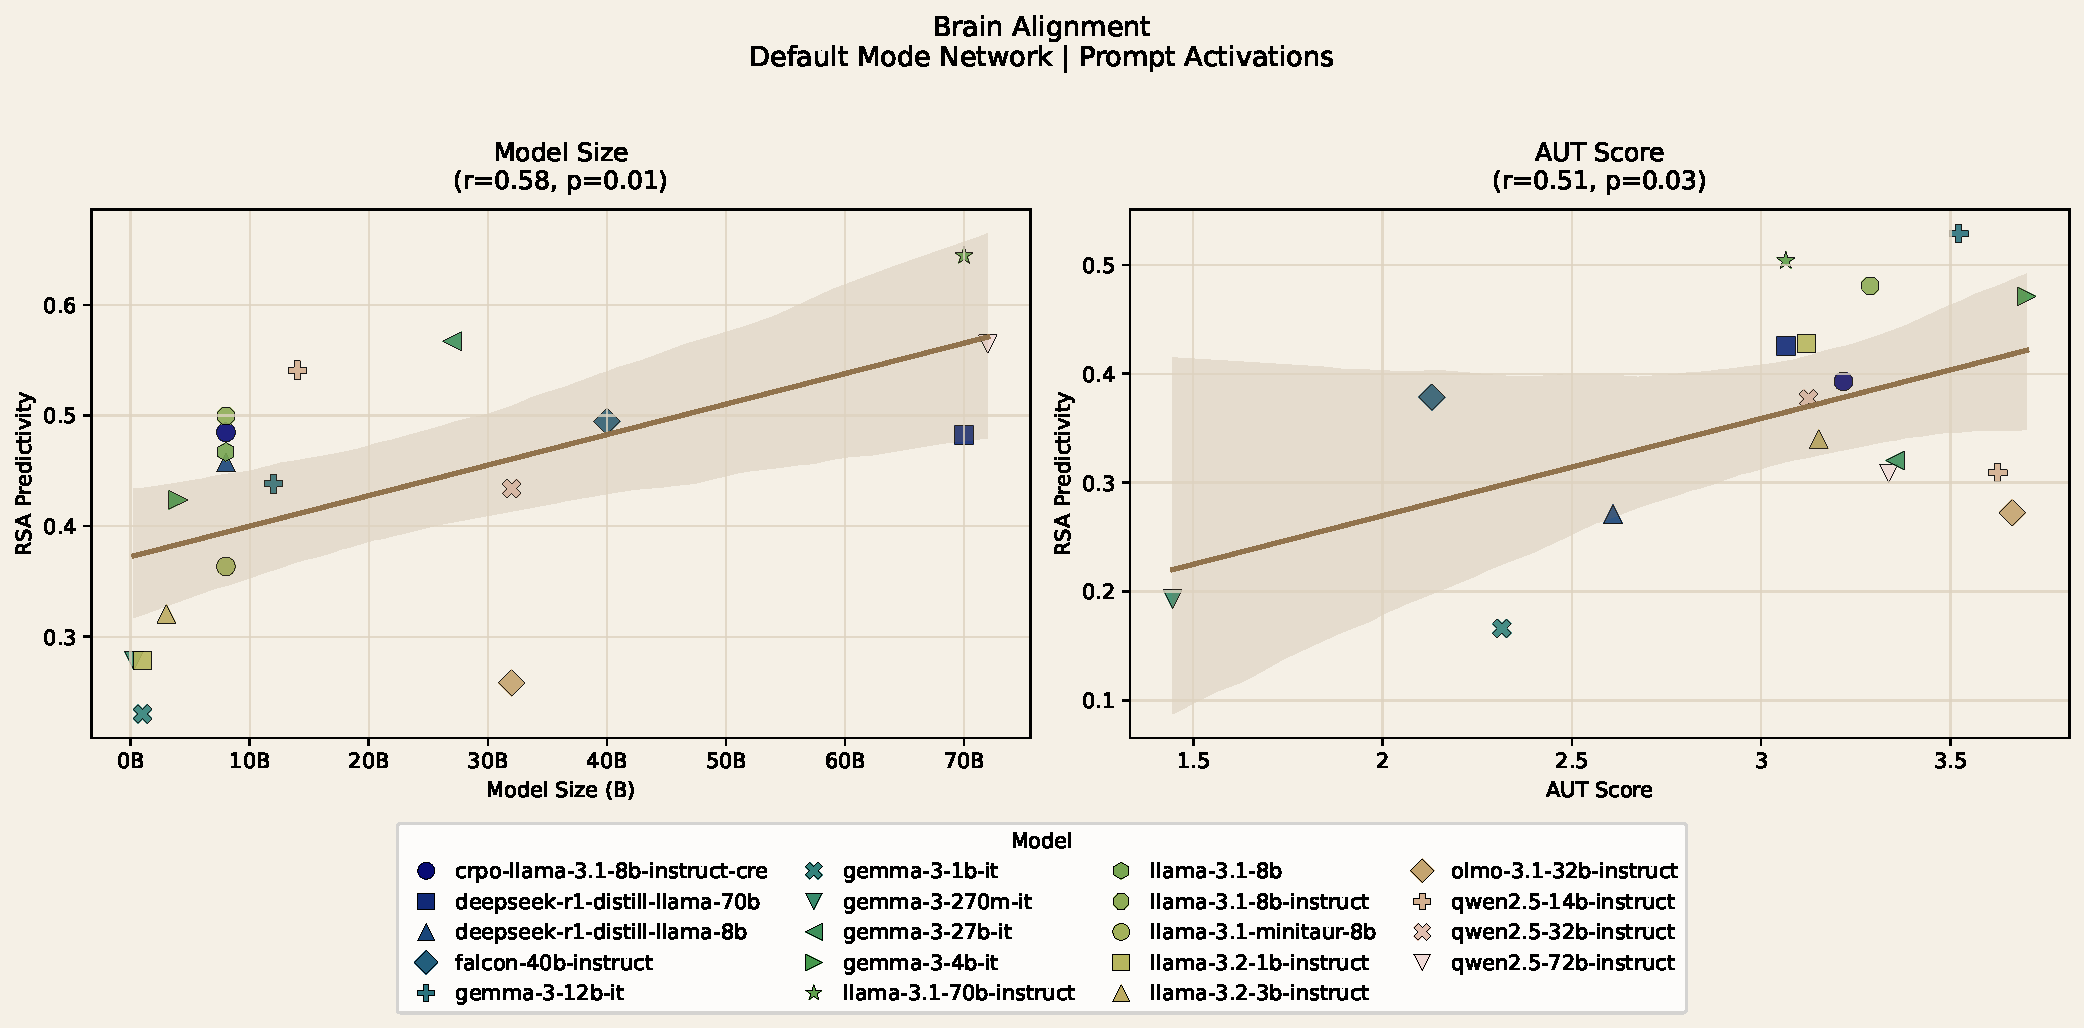
\includegraphics[width=\linewidth]{figures/main_results_yeo_dmn_prompt_nc0_t_1_t_mean.pdf}
\centering
\caption{\textbf{Default Mode Network (DMN) AUT brain alignment results by model size and task performance using model activations on stimuli (prompt) only.} $r$ and $p$ correspond to the Pearson correlation coefficient and p-value.}
\label{fig:alignment-aut-yeo-dmn-prompt}
\end{figure}

\subsection{Brain Alignment}
Brain alignment refers to the degree of similarity between the internal representations of an LLM and human neural activity \citep{schrimpf2018brain}. We evaluate alignment using Representational Similarity Analysis (RSA) \citep{kriegeskorte2008representational}. We note that while some past works have used linear predictivity (i.e., fitting a regression model to predict voxel-wise fMRI responses) \citep{schrimpf2018brain,schrimpf2021neural}, this metric typically requires a large sample of stimuli responses to be effective. While our data is large in terms of the number of subjects, the number of stimulus samples per subject is insufficient to train a meaningful regression model. Therefore, we opt not to use it in our alignment computation. 
% For linear predictivity, we fit a regression model to predict voxel-wise fMRI responses from LLM representations using k-fold cross-validation. At each fold, the fitted model is applied to held-out fMRI responses from the original corpus of recordings, and alignment is computed as the Pearson correlation between the predicted and actual responses. Correlations are then averaged across folds, yielding a per-voxel alignment score. 
To compute the RSA predictivity, we compare the geometry of representational dissimilarity matrices (RDMs) constructed from LLM representations and fMRI responses, respectively. We compute alignment at the level of individual subjects and report the median across subjects. To account for the inherent noise in fMRI measurements, we estimate a noise ceiling per subject, which represents the maximum alignment score achievable given the reliability of the neural data. Raw alignment scores are then divided by their corresponding noise ceilings, yielding noise-ceiling-normalized scores that allow for more meaningful comparisons across brain regions and models. We evaluate alignment at every layer of each LLM and take the maximum value across layers as the model's overall brain alignment score, following \citet{schrimpf2018brain}. This layer-selection procedure is motivated by the observation that different layers of a network capture different levels of representational abstraction and allow each model to be assessed at its most brain-aligned processing stage \citep{elhage2021mathematical, tenney2019bert, jawahar-etal-2019-bert}.

% \subsection{Localizing LLM Creativity Networks}
% In addition to examining alignment within individual model layers, we also employ functional localization to identify data-driven creativity networks in the LLM representations. 
% For the brain, we leverage the OCT task as a low-creativity control condition and perform a group-level GLM across subjects to compute the contrast between neural responses to AUT and OCT stimuli, expressed as z-scores. A threshold is then applied to this contrast map to identify a set of voxels that are selectively and reliably recruited during creative thinking, yielding a functionally defined brain creativity network. Figure \ref{fig:brain-custom-cre} shows the resulting network atlas. 
% We follow the approach previously used to identify the language network in language models \citet{alkhamissi2025llm, fedorenko2010new} and steer models to amplify creativity \citep{olson2024steering} and extract representations for both AUT and OCT stimuli and responses from each model. We then define the model's creativity network as the top-k units that maximally differentiate between the two conditions, identified by selecting units with the largest positive t-values from a Welch's t-test comparing activation magnitudes across AUT and OCT stimuli. This parallel localization procedure allows us to identify the most creativity-selective components of the model, and to examine their alignment in a functionally grounded manner.

% \begin{figure}[t]
% \includegraphics[width=\linewidth]{figures/aut_sub_oct_slm_z_score_th6.png}
% \centering
% \caption{Brain creativity network.}
% \label{fig:brain-custom-cre}
% \end{figure}


\subsection{Alignment with High vs. Low Creativity Responses}
\label{sec:high-low}
Prior work has shown that instruction tuning improves LLM alignment with the human language system \citep{aw2023instruction}, raising the question of whether different post-training approaches, such as those targeting creativity, human behavioral simulation, or reasoning, can selectively modulate alignment with neural responses associated with creative ideation. To explore this, we partition the human brain data into high- and low-creativity populations based on the mean human creativity rating assigned to each response. For each AUT stimulus, participant responses were rated on their creativity by four independent human raters ($ICC =0.75$, good inter-rater agreement), and we followed a standard practice to aggregate these scores by averaging to yield a single creativity score per response \citep{organisciak2023beyond, amabile1982social}. Since responses are rated on a scale of 1 to 5 and the mean rating distribution is left-skewed (Appendix Figure \ref{fig:dist-mean-rating}), to roughly match the number of samples between two conditions, we use a cutoff of $2.0$ to define low-creativity responses ($rating < 2.0$; $N=1,978$) and high-creativity responses ($rating \ge 2.0$; $N=1,358$).

\begin{figure}[t]
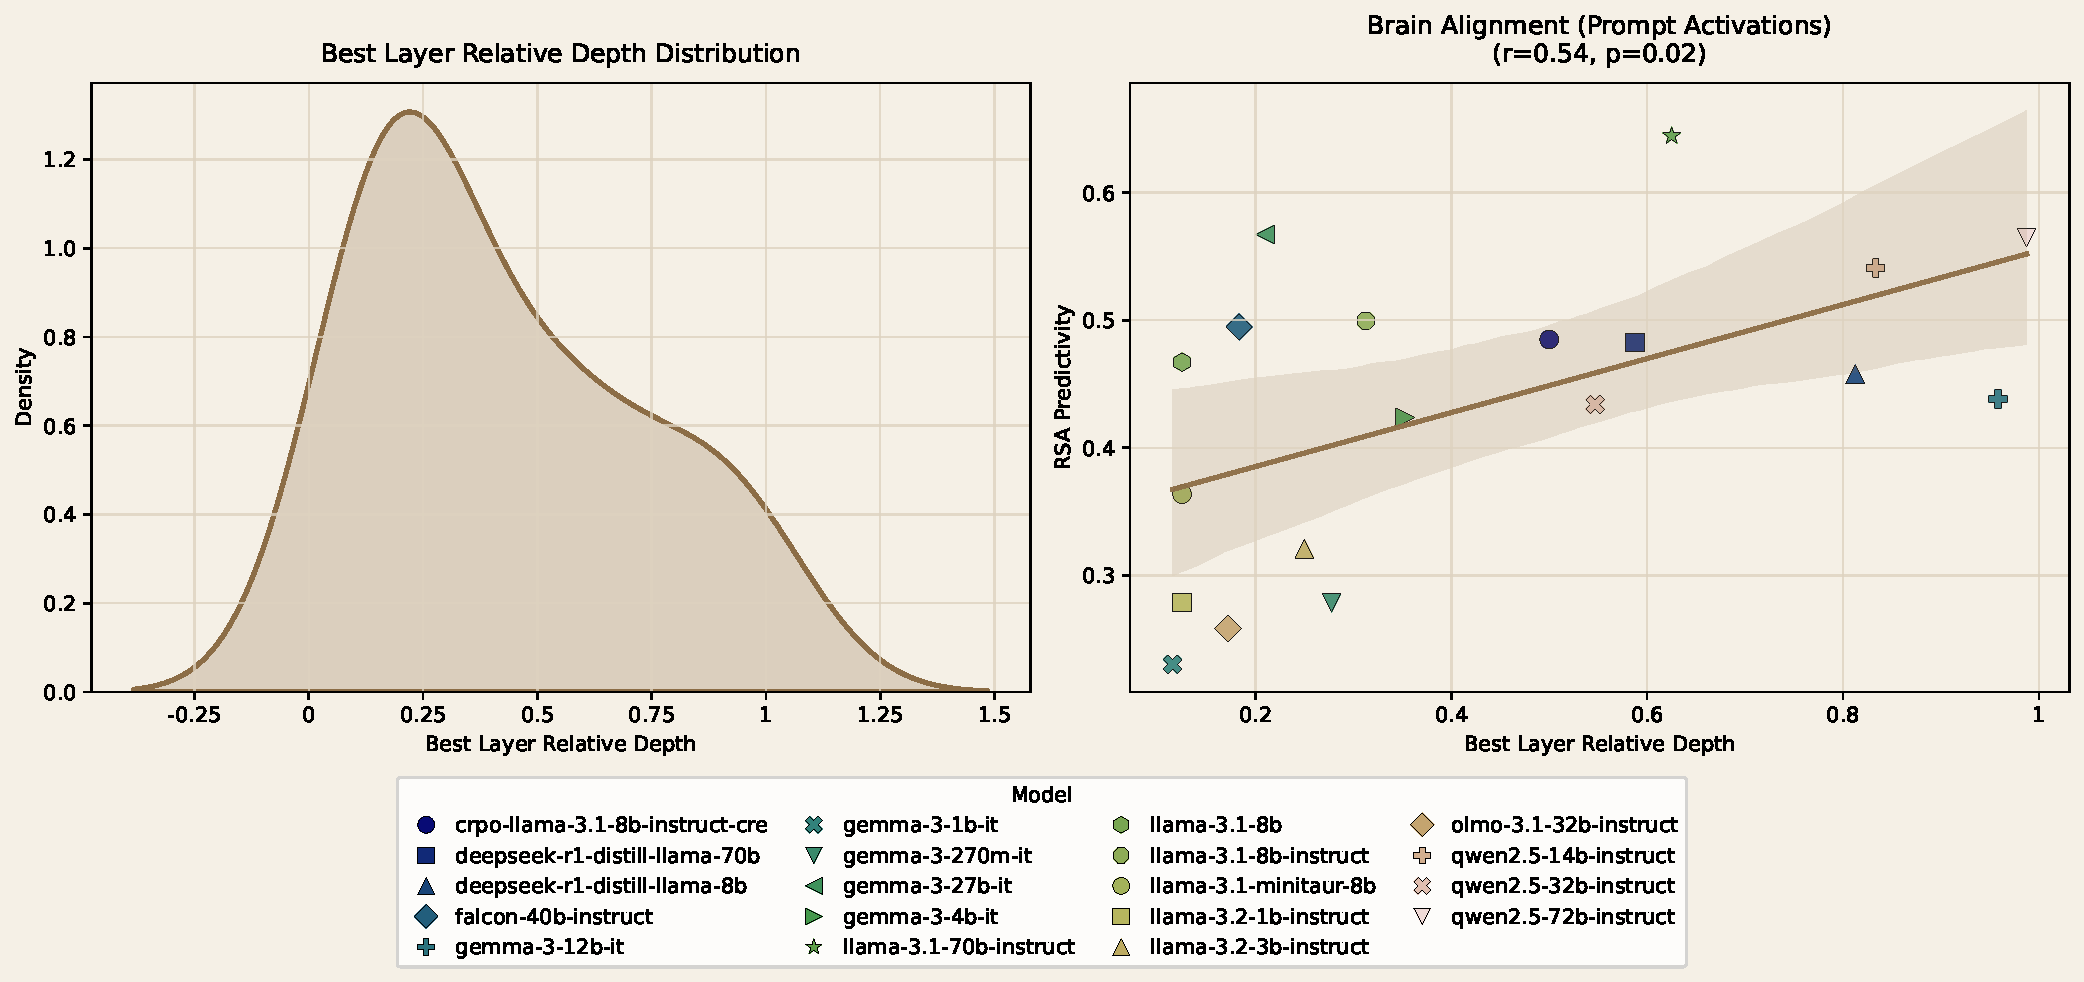
\includegraphics[width=\linewidth]{figures/best_layer_res_yeo_dmn_aut_prompt_nc0_t_1.pdf}
\centering
\caption{\textbf{Left:} The distribution of the best model layer (measured as relative depth) for alignment. \textbf{Right:} Default Mode Network (DMN) brain alignment results by best layer relative depth using model activations on stimuli (prompt) only.}
\label{fig:alignment-best-layer-aut-yeo-dmn}
\end{figure}

% To further probe the nature of brain-LLM alignment in divergent thinking, we investigate whether model representations are differentially aligned to neural responses associated with high versus low creativity ideation.
% This analysis allows us to ask a more fine-grained question than overall alignment: do LLMs, and in particular more creative LLMs, preferentially align to the neural representations underlying genuinely creative ideation, or is their alignment driven equally by routine, low-creativity responses? 
% If more creative models show disproportionately higher alignment to high-creativity brain responses, this would suggest that the representational geometry of creative LLM processing is specifically more similar to the neural geometry of human creative thought, rather than reflecting a general improvement in language processing. This would provide stronger evidence for a functionally meaningful correspondence between LLM creativity and human creative cognition at the neural level.